\documentclass[twocolumn,           % Format : preprint, twocolumn
%\documentclass[preprint,           % Format : preprint, twocolumn
               showpacs,            % Pacs : showpacs, noshowpacs
               preprintnumbers,     % Preprint: preprintnumbers,
               			    %           nopreprintnumbers
               aps,                 % Society: ...
               prl,          	    % Journal Style : pra, prb, prc, prd, pre,
               			    %                 prl, prstab, rmp
               letterpaper,             % Size : a4paper, ...
               superscriptaddress,      % Affiliation (Title) : groupedaddress,
                                    %                       superscriptaddress,
                                    %                       unsortedaddress
               nofootinbib,         % Footnote: footinbib, nofootinbib
               tightenlines,        % Remove additional spaces in a line
               floats,floatfix      % Floating pictures and tables
               ,usenatbib,
               ]{revtex4-1}
\usepackage{graphicx}  % needed for figures
\usepackage{dcolumn}   % needed for some tables}
%\usepackage[style=authoryear,backend=biber]{biblatex}
\usepackage{bm}        % for math
\usepackage{amsmath,amssymb}
\usepackage{hyperref}
\usepackage{color}
\definecolor{purple}{rgb}{0.58,0.0,0.83}
\usepackage{caption}
\usepackage[toc,page]{appendix}
\usepackage{subcaption}

\begin{document}

\title{Constraining two field inflationary models}
\author{Luis Padilla-Albores}  
\email{epadilla@fis.cinvestav.mx}
\affiliation{Departamento de F\'isica, Centro de Investigaci\'on y de Estudios Avanzados del IPN, A.P. 14-740, 07000 M\'exico D.F.,
  M\'exico.}
   \author{Jos\'e Alberto V\'azquez Gonz\'alez}  
\email{javazquez@icf.unam.mx}
\affiliation{Instituto de ciencias físicas, Universidad Nacional Aut\'onoma de M\'exico, sede Cuernavaca, Morelos, México}
\author{Tonatiuh Matos}  
\email{tmatos@fis.cinvestav.mx}
\affiliation{Departamento de F\'isica, Centro de Investigaci\'on y de Estudios Avanzados del IPN, A.P. 14-740, 07000 M\'exico D.F.,
  M\'exico.}
\date{\today}

\begin{abstract}
XX\\
XX\\
XX\\

\end{abstract}
\pacs{????}
\begin{keywords}
dark matter  -- galaxy clusters --  gravitation  -- relativity
\end{keywords}

\maketitle



\section{Introduction}
\label{introduction}

XXXXX

XXXXX

XXXXX

XXXXX

XXXXX

\section{Generalities for two field inflationary models}

Although one scalar field models for inflation can be preferable given the fact that they predict only adiabatic like perturbations, two field models can be interesting since there are some regions of parameters were this models can generate small isocurvature perturbations and the addition of new free parameters can help to ''death" single-field inflationary models to bring them back.  

In this section we review in a general way two field inflationary models for inflation following (Ref. Christian T. Byrnes and David Wands). 

\subsection{Background equation of motion}

In this section we consider a two-field inflationary model with canonical kinetic term and where its dynamics is described by an arbitrary interaction potential $V(\phi,\psi)$. As usual we consider that the classical fields are homogeneous and evolve in a FLRW background. Then, the background equation of motion for each scalar field and the Hubble parameter are
\begin{subequations}
\begin{equation}
\ddot{\phi}_i+3H\dot{\phi_i}+V_i=0 \ \ \ (i=\phi,\psi)
\end{equation}
\begin{equation}
H^2=\frac{8\pi G}{3}\left[V+\frac{1}{2}\left(\dot{\phi}+\dot\psi\right)\right],
\end{equation}
\end{subequations}
where $V_i\equiv\partial V/\partial \phi_i$. In the inflationary era it is usually assumed that the scalar fields are slow-rolling. This happens always that the condition $\epsilon_i,|\eta_{ij}|\ll 1$ is fulfill; $\epsilon_i$ and $\eta_{ij}$ are called the slow-roll parameters and are defined in appendix [A]. If this happens we can rewrite the above equations as
\begin{subequations}
\begin{equation}
\dot{\phi}_i\simeq \frac{2}{3}\epsilon_i V
\end{equation}
\begin{equation}
H^2\simeq \frac{8\pi G}{3}V\left(1+\frac{1}{3}\epsilon^H\right)
\end{equation}
\end{subequations}
where $\epsilon^H$ are new slow-roll parameters defined in appendix [A]. 
\subsection{The adiabatic and isocurvature perturbations}

The equation of motion for the perturbed fields in the spatially flat gauge are (ref)
\begin{equation}
\ddot{\delta\phi}_i+3H\dot{\delta\phi}_i+\sum_j\left[V_{ij}-\frac{8\pi G}{a^3}\frac{d}{dt}\left(\frac{a^3}{H}\dot{\phi}_i \dot\phi_j\right)\right]\delta\phi_j=0
\end{equation}
For the large scales ($k\ll aH$) it is better to work in a rotating basis of the fields given by
  \begin{subequations}
  \begin{equation}
  \binom{\delta \sigma}{\delta s}=S^{\dagger}\binom{\delta \phi}{\delta\psi}
  \end{equation}
  where
  \begin{equation}
  S=\begin{pmatrix}\cos\theta & -\sin\theta\\ \sin\theta & \cos\theta\end{pmatrix}, \ \ \ \tan\theta =\frac{\dot \psi}{\dot \phi}\simeq\pm \sqrt{\frac{\epsilon_\psi}{\epsilon_\phi}}
  \end{equation} 
  \end{subequations}
The field $\sigma$ is parallel to the trajectory and is usually called \textit{adiabatic field} while the field  $s$ is perpendicular to it and is called \textit{entropy field}. 

 If the background trajectory is curved it happens that $\delta\sigma$ and $\delta s$ are correlated at Hubble exit. In this way the power spectrum and cross-correlation at Hubble exit is given by
\begin{subequations}
\begin{equation}
P_{\sigma^*}((k))\simeq\left(\frac{H_*}{2\pi}\right)^2(1+(-2+6C)\epsilon-2C\eta_{\sigma\sigma})
\end{equation}
\begin{equation}
C_{\sigma s^*}(k)\simeq-2C\eta_{\sigma s}\left(\frac{H_*}{2\pi}\right)^2
\end{equation}
\begin{equation}\label{5c}
P_{s^*}(k)\simeq\left(\frac{H_*}{2\pi}\right)^2(1+(-2+2C)\epsilon-2C\eta_{ss})
\end{equation}
\end{subequations}
where $C\simeq 0.7296$ and $\epsilon$ and $\eta_{ij}$ ($i,j=\sigma,s$) are new slow-roll parameters defined in term of the new adiabatic and entropy fields (see appendix [A]).
\subsection{Final power spectrum and spectral index}
The curvature and isocurvature perturbations are defined as
\begin{equation}\label{RS}
R\equiv\frac{H}{\dot\sigma}\delta \sigma, \ \ \ S=\frac{H}{\dot \sigma}\delta s
\end{equation}
In the slow-roll limit in large scales, the evolution of curvature and isocurvature perturbations can be written using the formalism of tranfer matrix (ref) as
\begin{equation}
\binom{R }{S}=\begin{pmatrix}1 & T_{RS}\\ 0& T_{SS}\end{pmatrix}\binom{R}{S}_*
\end{equation}
where
\begin{subequations}
\begin{equation}
T_{SS}(t^*,t)=\exp\left(\int^t_{t^*}\beta Hdt'\right), \ \ \
\end{equation}
\begin{equation}\label{TRS}
T_{RS}(t^*,t)=\exp\left(\int^t_{t^*}\alpha T_{SS}Hdt'\right)
\end{equation}
\end{subequations}
and at linear order in slow-roll parameters
\begin{equation}
\alpha\simeq -2\eta_{\sigma s}, \ \ \ \ \beta\simeq-2\epsilon+\eta_{\sigma\sigma}-\eta_{ss}
\end{equation}

In the other side the primordial curvature perturbation, during radiaton-dominates era some time after inflation has ended, is given in large scales by
\begin{equation}
R=\Psi+\frac{H\delta\rho}{\rho}
\end{equation}
where $\Psi$ is the gravitational potential. The conventional definition of the isocurvature perturbation for an $i$ specie is given relative to the radiation density by
\begin{equation}
S_i=H\left(\frac{\delta\rho_{i}}{\rho_{i}}-\frac{\delta\rho_\gamma}{\rho_\gamma}\right).
\end{equation}
Then, the final power spectrum at the beginning of the radiation-domination era is given by
\begin{subequations}\label{spectrums}
\begin{equation}\label{PRf}
P_R\simeq P|_*(1+\cot^2\Delta),
\end{equation}
\begin{equation}
P_S=T^2_{SS}P|_*,
\end{equation}
\begin{equation}
C_{RS}=T_{RS}T_{SS}P_R|_*
\end{equation}
\end{subequations}
where at linear order in slow-roll parameters
\begin{equation}
P|_*=\frac{1}{2\epsilon}\left(\frac{H_*}{2\pi M_{pl}}\right)^2
\end{equation}
with $M_{pl}$ the Planck mass and $\Delta$ is the observable correlation angle defined at lower order as
\begin{equation}
\cos\Delta =\frac{T_{RS}}{\sqrt{1+T_{RS}^2}}.
\end{equation}
The final scalar tilts, defined as $n_x-1=d\ln P_x/d\ln k$, at linear order in slow-roll parameters are
\begin{subequations}\label{tilts}
\begin{eqnarray}
n_R-1&\simeq & -(6-4\cos^2\Delta)\epsilon+2\sin^2\Delta\eta_{\sigma\sigma}\nonumber \\ &&+4\sin\Delta\cos\Delta\eta_{\sigma s}+2\cos^2\Delta\eta_{ss}\\
n_c-1&\simeq &-2\epsilon+2\tan\Delta\eta_{\sigma s}+2\eta_{ss}\\
n_S-1&\simeq & -2\epsilon+2\eta_{ss}
\end{eqnarray}
\end{subequations}

In order to understand what is the contribution of our dark matter candidate to the primordial spectrum, it is better to rewritte the primordial adiabatic and entropy perturbations on super-horizon scales as a power law, given by
\begin{subequations}\label{PswAs}
\begin{equation}\label{PrAs}
P_R=A_r^2\left(\frac{k}{k_0}\right)^{n_{ad1}-1}+A_s^2\left(\frac{k}{k_0}\right)^{n_{ad2}-1}
\end{equation}
\begin{equation}\label{PrCrs}
C_{RS}=A_SB\left(\frac{k}{k_0}\right)^{n_{cor}-1}
\end{equation}
\begin{equation}\label{PsAs}
P_s=B^2\left(\frac{k}{k_0}\right)^{n_{iso}-1}
\end{equation}
\end{subequations}
where at linear order $n_{ad1}=-6\epsilon+2\eta_{\sigma\sigma}$, $n_{ad2}=2n_C-n_S$, $n_{cor}=n_c$, $n_{iso}=n_S$. We have that $A_r^2$, $A_s^2$ and $B$ can be written in terms of the correlation angle as
\begin{subequations}
\label{RelAs}
\begin{equation}
A_r^2=[P_R\sin^2\Delta]_{k_0}, \ \ \ \ A_s^2=[P_R\cos^2\Delta]_{k_0},
\end{equation}
\begin{equation}
B^2=[T_{SS}^2 P_R|_*]_{k_0}
\end{equation}
\end{subequations}
$A_r^2$ and $A_s^2$ are the contribution of the adiabatic and entropy fields to the amplitud of the primordial adiabatic spectrum. 
\subsection{Gravitational waves}

Given the fact that scalar and tensor perturbations are decoupled at linear order, the gravitational waves at horizon crossing is the same than in the case of a single field and the amplitude of gravitational waves remains frozen-in on large scales after Hubble exit during inflation. In this way the power spectrum and the tilt of the gravitational waves is given by
\begin{equation}
P_T=P_{T*}\simeq 8 \left(\frac{H_*}{2\pi M_{pl}}\right)^2(1+2(-1+C)\epsilon)
\end{equation}
\begin{equation}\label{tiltsnt}
n_T\simeq -2\epsilon\left[1+\left(\frac{4}{3}+4C\right)\epsilon+\left(\frac{2}{3}+2C\right)\eta_{\sigma\sigma}\right]
\end{equation}

The tensor-to-scalar ratio at Hubble exit is the same than in the single field. However, at super-horizon scales, the curvature perturbations continue evolving as \eqref{PRf}. In this way the tensor-to-scalar ratio some time after the end of inflation is
\begin{equation}\label{Tensortoscalar}
r\simeq 16\epsilon \sin^2\Delta\left[1-\left(\frac{4}{3}+4C\right)\epsilon +\left(\frac{2}{3}+2C\right)\eta_{\sigma\sigma}\right]
\end{equation}
\section{Experimental constraints for inflationary parameters}

\textcolor{red}{Meter aqu\'i las constricciones experimentales que hay con Planck.}

%
%
%
%
%
%
\section{Simplest scenario: The single field straight scenario and constraints for SFDM models}

The simplest scenario is to consider that only one scalar field was dynamically important during inflation and the extra scalar field observer contributed to the primordial spectrum by generating only isocurvature fluctuations. Even tough the idea of adding an extra spectator that does not contribute for inflation could be considered as no necessary, there are at least two scenarios where this extra degrees of freedom can be important. First is the so called curvaton inflationary model (ref), where it is consider that this new field is responsible for the majority of the adiabatic perturbations produced during inflation. This scenario has been well studied in the literature (ref) and now a days it is one of the preferable scenarios for inflation (ref). In the other side we can consider an scenario where this extra scalar field can be used as a Dark Matter candidate, in such case we will have isocurvature constraints for our model. 

\subsection{SFDM spectator scenario}
The idea of scalar fields as the DM of the Universe was first suggested in (Baldeshti et al. (1983)) and rediscovery by various authors with different names (see e.g. Membrado et al. 1989; Press et al. 1990; Sin 1994; Ji $\&$ Sin 1994; Lee $\&$ Koh 1996; Sahni $\&$ Wang 2000; Peebles 2000; Goodman 2000; Matos $\&$ Ure\~na-L\'opez 2000; Matos $\&$ Arturo Ure\~na-L\'opez 2001; Wetterich 2001; Arbey et al 2001; Woo $\&$ Chiueh 2009; Lundgren et al. 2010; Calabrese $\&$ Spergel 2016; Schwabe et al. 2016; Hui et al. 2017; Moez et al. 2017, among others), for example: SFDM (Matos $\&$ Guzm\'an 2000), fuzzy DM (HU et al. 2000), wave DM (Bray 2010; Schive et al. 2014a), Bose-Einstein condensate DM (B\"omer $\&$ Harko 2007) or ultra-light axion DM (Marsh $\&$ Ferreira 2010). \textcolor{red}{(Completar este p\'arrafo diciendo que el modelo es un candidato serio y meter m\'as referencias).} 


In this scenario we need that the SFDM candidate being a stable spectator field and that its classical dynamics during inflation being negligible. We can obtain such scenario by considering that the trajectory in the field space evolves in the inflaton direction $\phi$ whereas the direction perpendicular to the trajectory corresponds with the SFDM $\psi$. Notice that it is necessary to have $\eta_{\sigma s}=\eta_{\psi\phi}=0$ and that our dark matter candidate evolves much slower than the inflaton. Then, we can see that the last conditions demand that the potential can be written as $V(\phi,\psi)=V(\phi)+V(\psi)$ and $\epsilon_\psi\ll \epsilon_\phi$.

During the inflationary scenario the entropy and adiabatic perturbations are uncorrelated which implies that $T_{RS}=0$ (and $C_{RS}=0$) as can be seen from \eqref{TRS} imposing initial conditions at horizon crossing. In this way we have that $\cos\Delta =0$. 

As is expected from \eqref{PrAs} and \eqref{RelAs} in the inflationary scenario the primordial power spectrum for the adiabatic perturbations is produced purely by the inflaton while quantum fluctuations of the scalar field dark matter give entry to the generation of uncorrelated isocurvature perturbations. In this way the primordial power spectrum of adiabatic, isocurvature and tensor perturbations are
\begin{subequations}
\begin{equation}
P_R=P_R|_*
\end{equation}
\begin{equation}\label{PS1}
P_s=T_{SS}^2 P_R|_*
\end{equation}
\begin{equation}
P_T=\frac{8}{M_{pl}^2}\left(\frac{H_*}{2\pi}\right)^2
\end{equation}
\end{subequations}
and from \eqref{tilts} and \eqref{tiltsnt} the tilts at linear order are
\begin{subequations}
\begin{equation}
n_R\simeq-6\epsilon+2\eta_{\phi\phi}
\end{equation}
\begin{equation}
n_s\simeq-2\epsilon+2\eta_{\psi\psi}
\end{equation}
\begin{equation}
n_T\simeq -2\epsilon
\end{equation}
\end{subequations}
Finally the tensor-to-scalar ratio in this scenario is the same than in the single-inflaton scenario
\begin{equation}
r\simeq 16\epsilon
\end{equation}
which implies that the SFDM observer does not contribute to $r$.

The adiabatic scalar amplitude of perturbations generated during inflation is (ref) 
$A_r^2=2.19\times 10^{-9}
$ which implies that the perturbations for the scalar field dark matter in this scenario is given by $B^2=2.19\times 10^{-9}T_{SS}^2$ where $T_{ss}^2$ depends of the model of inflation that we are considering. It happens that in exactly de-sitter inflation $\epsilon\sim 0$ we have $T_{SS}^2=1$. 

\subsubsection{Initial condition from inflation and constraining isocurvature perturbations}

In this scenario and considering that the dark matter is only composed of SFDM, the perturbation evolution for photons, neutrinos, barions and dark matter start from the initial conditions $\frac{3}{4}\delta_{\gamma}=\frac{3}{4}\delta_\nu=\delta_b\simeq 0$ and $\delta_{SFDM}=A_{SFDM}$ where $\delta_{\alpha}=\delta \rho_\alpha/\rho_\alpha$ and $A_{SFDM}$ is the gauge invariant entropy perturbation
\begin{equation}
A_{SFDM}=\delta_{SFDM}-3\frac{\delta T}{T}
\end{equation}
The fact that $\delta_{SFDM}\gg \delta_{\gamma}$ implies that $\delta_{SFDM}\gg 4\delta T/T$ and then $A_{SFDM}=\delta_{SFDM}$. Notice, from \textcolor{red}{(eq)}, that $\rho_{SFDM}\propto |\psi|^2$ and then we can rewrite $\delta_{SFDM}$ as 
$\delta_{SFDM} = 2\delta \psi/\psi_i
$,
where $\psi_i$ is the SFDM background value during inflation. In this way we can obtain a primordial isocurvature perturbation for a SFDM candidate as
\begin{equation}
P_{SFDM}(k)=\left(\frac{H_*}{\pi \psi_i}\right)^2
\end{equation}

Since SFDM behaves similar to LCDM at cosmological levels, the CMB constraints on CDM isocurvature perturbations applies to SFDM as well. By relating the isocurvature power spectrum with the curvature power as
\begin{equation}
P_{SFDM}(k)=\frac{\beta_{iso}(k)}{1-\beta_{iso}(k)}P_R(k)
\end{equation}
we obtain constraints given by Planck (ref) at the pivot scale $k_0/a_0=0.05Mpc^{-1}$ and for uncorrelated and scale-invariant isocurvature perturbations 
\begin{equation}
\beta_{iso}(k_0)<0.038 \ \ \ \ \ (95\%\ \ \text{C.L., TT, TE, EE$+$lowP})
\end{equation}
This last expression can be extrapolated to impose upper constraints to the mass for our SFDM candidate in terms of the upper limit of the tensor to scalar ratio (see (ref))
\begin{equation}
r<2\times 10^{-4}\left(\frac{g_{*osc}}{3.36}\right)^{-3/4}\left(\frac{g_{s*osc}}{3.91}\right)\left(\frac{m}{10^{-22}}\right)^{-1/2}
\end{equation}
where $g_{*osc}$ and $g_{s*osc}$ are the number of degrees of freedom at SFDM and entropy oscilations. Given that our SFDM candidate starts its oscilation at radiation-domination epoch (when its mass $m\sim H$), we can take $g_{*osc}=3.36$. Taking $g_{s*osc}=3.91$ we can obtain a direct constrain for the scalar field mass for inflation as 
\begin{equation}
\frac{m}{10^{-22}\ eV}<\left(\frac{2\times 10^{-4}}{r}\right)^2
\end{equation}

In ref. (ref) it was obtained the above expression thinking in the SFDM candidate as an axion-like particle, it is, a field that is created by a missalignment mechanism. However, we can see that such result can be extrapolated for whichever SFDM candidate as general constraints for it if the scalar field coexist with the inflaton. We can observe in figure \ref{constraintsSFDM} such constraints in the m vs r plane. As we can see if $r$ is detected in the near future, it will ruled-out models where more massive scalar fields could coexist with the inflaton during inflation. This constraints are important given that in (ultra-light axion like DM must be presented during inflation) it was demonstrated that an ultra-light axion-like dark matter candidate must be presented during inflation. Then, if $r$ is detected in the near future, it could represent an strong constraint for the axion-like particle model. Notice that if we relax the scalar field mechanism under this particle is created, we should expect that this restrictions can be less affective to the model if we consider that the SFDM candidate was created after inflation. 

\begin{figure}
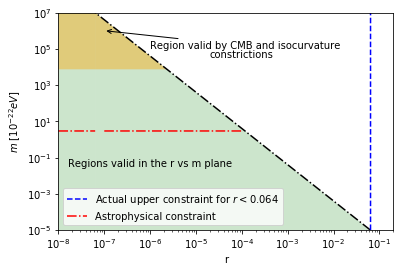
\includegraphics[width=8cm]{SFDMconstraints.png}
\caption{Isocurvature constraints for the SFDM candidate.}\label{constraintsSFDM}
\end{figure}

\subsection{Curvaton scenario}

In the curvaton scenario it is assumed that during inflation there was an extra scalar field that coexist with the inflaton and its classical dynamics was negligible (its energy density was sub-dominant during inflation). Then, similar to the SFDM scenario, this scalar field obtained quantum fluctuations, leading to the generation of primordial isocurvature perturbations. If the curvaton field is long lived (at least its life must be longer than the inflaton one) it starts to oscillate when the Hubble scale $H$ approaches the curvaton mass (see appendix [B]) shortly before or after the inflaton decays to radiation. During its oscillation phase, this curvaton field starts to behave as dust and then its perturbations are reduced slower than the ones associated with the inflaton [ref]. If the curvaton decays to radiation when its quantum fluctuations dominates over the inflaton ones, we can obtain a scenario where curvaton quantum fluctuations can dominate the early Universe and give place to be the totality of the initial adiabatic perturbations (ref). In our formalism, such scenario is obtained when $T_{RS}>>1$ or equivalently when we consider in our analysis $\sin\Delta = 0$ (ref), in such case we obtain that the tensor-to-scalar ratio in the pure curvaton scenario is $r=0$.  

In the last few years people has started to study curvaton models but considering that the curvaton field does not constribute for the totality of the primordial adiabatic perturbations, instead, it contributes to a fraction of the total curvature perturbations, while the remaining one was produced by the inflaton (ref). Notice that such scenario is obtained if $0<\cos\Delta <1$. It is also usual to redefine a new parameter in this model $R= [\cot^2\Delta]_{k_0}$ which can be related with the curvaton-to-inflaton density fraction of primordial curvature perturbations. Then, the primordial adiabatic perturbations can be written from \eqref{PrAs} as
\begin{equation}\label{PCr}
\mathcal{P}_R(k)=A_r\left(\left(\frac{k}{k_{0}}\right)^{n_s^\phi-1}+R\left(\frac{k}{k_{0}}\right)^{n_s^\psi-1}\right)
\end{equation}
where $n_s^\phi-1 = -6\epsilon_\phi+2\eta_{\phi\phi}$ and $n_s^\psi-1 = -2\epsilon_\psi+2\eta_{\psi\psi}$.
The total spectral index ($n_s-1=d\ln P_R/d\ln k$) is given then by
\begin{equation}
n_s-1=\frac{n_s^\phi+R n_s^\psi}{1+R}-1
\end{equation}

An advantage of this kind of models is that it can help to single inflationary models that at the moment could be considered as ruled-out by the data (but that could be well motivated theoretically) to remain in the competition in the inflationary zoo. As an example in (referencia de Curvaton after Planck) it was studied in a Bayesian framework several inflationary models with an extra light scalar field with a quadratic-like potential \textcolor{red}{(Checar bien esta parte)}. In such study it was obtained that one of the most preferable scenarios is a quartic-like inflationary potential with our extra scalar spectator. However it is necessary to notice that such scenario is favorable only in the limit where the curvaton produced nearly the totality of the primordial adiabatic perturbations, i.e. when $R>>1$. If in the other side we allow that our parameter $R$ takes whichever value, we could expect that more chaotic-like inflationary potentials could continue fitting observations. In fact when we consider the chaotic potential $V(\phi)=(1/2)m_p\phi^p$ for the inflaton and the  potential $V(\psi)= (1/2)M^2\psi^2$ for the curvaton, the spectral index $n_s$ is rewritten as
\begin{equation}
\label{nsexplicit}
n_s-1\approx -\frac{1}{1+R}\frac{2(2+p)}{4N+p}+\frac{R}{1+R}\left[-\frac{2p}{4N+p}+\frac{2M^2}{3H_*^2}\right]
\end{equation}
where  $N$ is the number of e-folds produced before our scales left the horizon and it is usually used $N=50\sim 60$. In the above equation we have used the Friedman equation in the slow-roll approximation for the term containing $M$. In this way from \eqref{Tensortoscalar} the tensor to scalar ratio in this model is given by
\begin{equation}\label{tensortoscalar}
r=\frac{16\epsilon_\phi}{1+R}
\end{equation}		
If we use \eqref{tensortoscalar} into \eqref{nsexplicit} we have 
\begin{equation}
n_s-1=-\frac{(2+p)}{8p}r+\left[1-\frac{(4N+p)}{16p}r\right]\left[\frac{2}{3}\frac{M^2}{H^2}-\frac{2p}{4N+p}\right]
\end{equation}
where we have obtained a relation between the spectral index and the tensor-to-scalar ratio which are well constrain by the data. Notice that in the limit when the curvaton dominates completely the adiabatic perturbations ($r\simeq 0$) and considering the mass of the curvaton negligible compared with the Hubble parameter (i.e. $M<<H$) we obtain that $n_s-1\simeq p/(120+p/2)$ and then the observational constrains for the spectral index means that the inflaton field must be close to be a quartic potential, $p=4$. Such result can be observed in figure \ref{nvsr}, where we have plotted the above equation neglecting $M/H$ and letting $R$ to vary using as our only constriction for it the actual upper constraint on $r$. In such figure we can observe an upper an lower value for $n_s$ in terms of $r$ which is obtained when we consider $N=60-50$ e-folds at the moment when our scales left the horizon. In the other side when we allow $M/H$ to vary using as our constriction that $M/H<1$ (in order to obtain quantum fluctuations for the curvaton during inflation) we can obtain that for some regions of parameters more chaotic like potentials can fit well the data. Such results can be observed in figures \ref{curv50} and \ref{curv60} where we have plotted contour plots for $r$ from the above equation in the $M/H$ vs $n_s$ plane. In this way we have seen the big advantage of adding this new degree of freedom to a simple chaotic-like model of inflation.
\begin{figure}
\centering
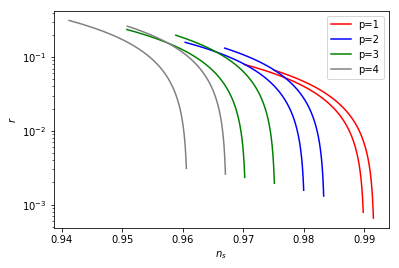
\includegraphics[width=0.4\textwidth]{nvsr}
\caption{Possible values in the n vs r plane when we allow $R$ to vary. The values that can be produced by the models are the ones between the two limits plotted in the figure.\textcolor{red}{(Tratar de pintar las regiones entre las l\'ineas y poner los datos de Planck para que se vea mejor.)}}
\label{nvsr}
\end{figure}
% * <epadilla@fis.cinvestav.mx> 2018-04-29T03:33:02.572Z:
%
% ^.
\newpage
\begin{figure}[h]
\centering
\begin{subfigure}[b]{\textwidth}
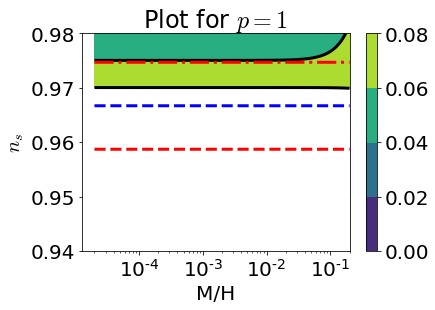
\includegraphics[width=0.4\textwidth]{p150.png}
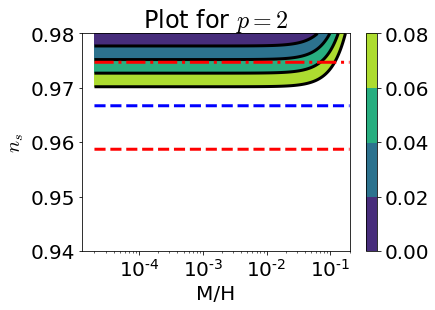
\includegraphics[width=0.4\textwidth]{p250.png}\\
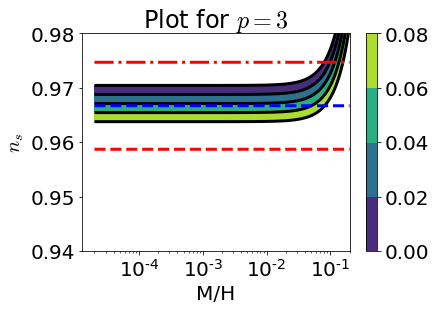
\includegraphics[width=0.4\textwidth]{p350.png}
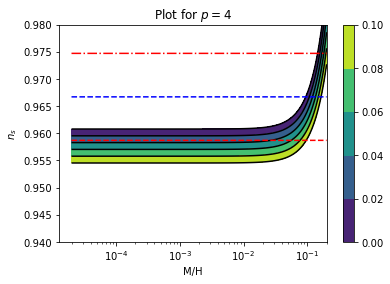
\includegraphics[width=0.4\textwidth]{p450.png}
\label{curv50}
\end{subfigure}
\caption{Inflationary constraints in the $M/H$ vs $n_s$ plane for $N=50$ e-folds. We plotted contour regions for $0<r<0.1$.}
\begin{subfigure}[b]{\textwidth}\centering
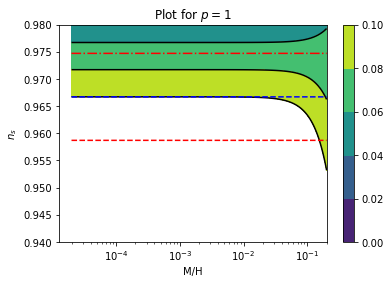
\includegraphics[width=0.4\textwidth]{p160.png}
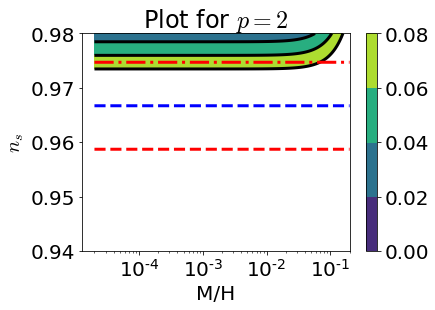
\includegraphics[width=0.4\textwidth]{p260.png}\\ 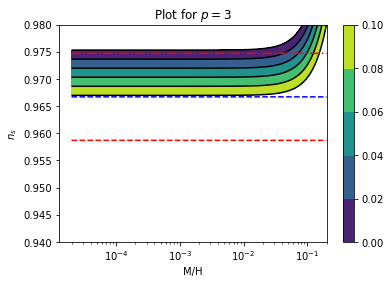
\includegraphics[width=0.4\textwidth]{p360.png}
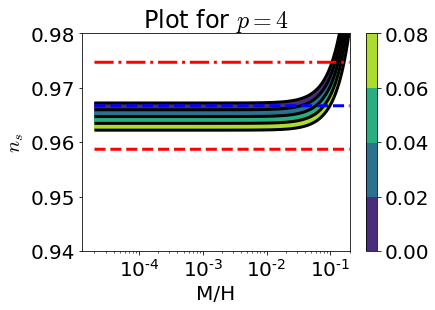
\includegraphics[width=0.4\textwidth]{p460.png}
%\captionof{figure}
%{\footnotesize{A }}
\label{curv60}
\end{subfigure}
\caption{Inflationary constraints in the $M/H$ vs $n_s$ plane for $N=60$ e-folds. We plotted contour regions for $0<r<0.1$.}
\end{figure}
\section{Constraining two field models with last data}
A
\section{Conclusions}
\appendix
\section{Slow-Roll index}

In this appendix we define the slow roll indexes used in our calculation. We have:
\begin{subequations}
\begin{equation}
\epsilon_i = \frac{1}{16 \pi G}\left(\frac{V_i}{V}\right)^2, \ \ \ \ \ \text{where $i=\phi,\psi$}
\end{equation}
\begin{equation}
\eta_{ij}=\frac{1}{8\pi G}\left(\frac{V_{ij}}{V}\right)
\end{equation}
\end{subequations}
where $V_i = \partial V/\partial \phi_i$. In the other side we have
\begin{equation}
\epsilon \equiv \frac{1}{16\pi G}\left(\frac{V_\sigma}{V}\right)^2\simeq \epsilon_\phi+\epsilon_\psi
\end{equation}
and
\begin{eqnarray}
\eta_{\sigma\sigma}&=&\eta_{\phi\phi}\cos^2\theta + 2\eta_{\phi\psi}\cos\theta\sin\theta+\eta_{\psi\psi}\sin^2\theta\nonumber \\
\eta_{\sigma s}&=&(\eta_{\psi\psi}-\eta_{\phi\phi})\sin\theta\cos\theta + \eta_{\phi\psi}(\cos^2\theta-\sin^2\theta)\\
\eta_{ss}&=&\eta_{\phi\phi}\sin^2\theta - 2\eta_{\phi\psi}\cos\theta\sin\theta+\eta_{\psi\psi}\cos^2\theta\nonumber 
\end{eqnarray}

\section{Papers}
Aqu\'i pondré de mientras los links de los papers que he revisado:

https://arxiv.org/pdf/1712.05364.pdf

https://arxiv.org/pdf/1505.00639.pdf

https://arxiv.org/pdf/astro-ph/0306500.pdf
\end{document}